
\chapter{Method 2: Tri-dexel}
\label{ch:tri_dexel}

The second discussed method to extract a triangulated surface from the VML's data model is based on a tri-dexel representation, \cf section \ref{sec:surface_representations}.
As observed with the previously shown method in chapter \ref{ch:direct_intersection}, reconstructing a surface directly form the many intersecting triangles stored in the VML's grid is computationally expensive, highly numerically unstable and prone to errors.
A more robust approach is desirable, which is able to always successfully reconstruct a surface with good quality.
This reconstruction should succeed independently of the complexity of the maintained geometry.
As a trade-off for this robustness, the approach may sacrifice surface exactness and filigree features.
Dexel-based representations fit this purpose nicely.
They provide a good abstraction of a machined workpiece with rich semantics.
The used grid resolution supplies an easy to configure level of detail and steering parameter between representation quality and memory/CPU demands.
Creating dexel-based representations from the VML's data model is achieved using an adaption of the already implemented, well-working and robust raycasting subsystem used for visualization, \cf section \ref{sec:raycasting}.
To achieve a good portrayal independently of the workpiece's orientation, three axis-aligned dexel images will be generated, thus creating a tri-dexel representation.
For converting such a tri-dexel model into a final triangle mesh, various algorithms are found in literature.
An excellent example is Ren \etal's "Feature Conservation and Conversion of Tri-dexel Volumetric Models to Polyhedral Surface Models for Product Prototyping" \cite{tridexel_reconstruction}.
Their approach form the idea and foundation of the implementation presented in this chapter.


\section{Concept}
\label{sec:tri_dexel_concept}

Firstly, a tri-dexel representation of the VML's data model has to be obtained.
Dexel images, in general, are created by sampling the workpiece's surface along parallel lines.
This sampling process is already implemented in the raycasting subsystem as part of the visualization.
However, when sampling dexels, a ray must not stop at the first surface intersection, but continue through the whole data model and collect all intersections along its path.
At each intersection, the intersection depth, \ie distance from the ray's origin, and the surface normal of the intersected triangle is recorded as a dexel node.
From the dexel's origin and a node's depth the intersection point can be calculated.
The raycast itself is performed with axis-parallel rays starting at equidistant origins from three sides of the VML's data model, thus creating three dexel images.
Combining these dexel images creates a uniform regular grid, the tri-dexel grid.
Figure \ref{fig:cylinder_head_dexel} shows the cylinder head scene with a low-resolution dexel image and the final reconstruction.

\begin{figure}
	\centering
	\begin{subfigure}[t]{0.3\textwidth}
		\centering
		\includegraphics[width=\textwidth]{images/cylinder_head_stock_and_svs}
		\caption{Stock and SVs}
		\label{fig:cylinder_head_stock_sv}
	\end{subfigure}
	\begin{subfigure}[t]{0.3\textwidth}
		\centering
		\includegraphics[width=\textwidth]{images/cylinder_head_vml}
		\caption{VML}
		\label{fig:cylinder_head_classified}
	\end{subfigure}
	\begin{subfigure}[t]{0.3\textwidth}
		\centering
		\includegraphics[width=\textwidth]{images/cylinder_head_dexel_image}
		\caption{Tri-dexel image}
		\label{fig:cylinder_head_dexel_image}
	\end{subfigure}
	\begin{subfigure}[t]{0.3\textwidth}
		\centering
		\includegraphics[width=\textwidth]{images/cylinder_head_dexel_image_center}
		\caption{Tri-dexel image center}
		\label{fig:cylinder_head_dexel_image_center}
	\end{subfigure}
	\begin{subfigure}[t]{0.3\textwidth}
		\centering
		\includegraphics[width=\textwidth]{images/cylinder_head_dexel_image_fins}
		\caption{Tri-dexel image fins}
		\label{fig:cylinder_head_dexel_image_fins}
	\end{subfigure}
	\begin{subfigure}[t]{0.3\textwidth}
		\centering
		\includegraphics[width=\textwidth]{images/cylinder_head_reconstructed}
		\caption{Result}
		\label{fig:cylinder_head_reconstructed}
	\end{subfigure}
	\caption{
		Tri-dexel based surface reconstruction from the VML's data model of a cylinder head.
		Figure \ref{fig:cylinder_head_stock_sv} shows the stock and a few swept volumes creating the fins and drillings.
		Figure \ref{fig:cylinder_head_classified} shows the classification result after these solids have been mapped into the VML's regular grid.
		The removed triangles are clearly visible, especially at the swept volumes.
		By using a raycast of axis parallel rays along all three coordinate system axes a tri-dexel representation is created as shown in figure \ref{fig:cylinder_head_dexel_image}.
		The resolution of the grid spawning the rays is 30 along the longest dimension.
		Figure \ref{fig:cylinder_head_dexel_image_center} and \ref{fig:cylinder_head_dexel_image_fins} show details of the tri-dexel image.
		The former views the drilling at the center from above and the latter views the cylinder head's fins from the center.
		Finally, the reconstructed surface is shown in figure \ref{fig:cylinder_head_reconstructed}.
		Note the imperfections at the fin's edges and bases.
	}
	\label{fig:cylinder_head_dexel}
\end{figure}

Secondly, the tri-dexel representation is converted into a triangle mesh.
This procedure is mostly based on the paper already mentioned during the introduction \cite{tridexel_reconstruction}.
Each intersection point of three orthogonal dexels from the tri-dexel grid forms a grid point.
If a grid point lies within a dexel segment on any of these dexels, it is said to be occupied, \ie lies within the workpiece's volume.
8 grid points and their 12 connecting edges along with their dexel segments are grouped into cells of the grid.
Each grid cell is then processed independently.
Figure \ref{fig:tri_dexel_cell} shows the structure of a tri-dexel cell.
%
\begin{figure}
	\centering
	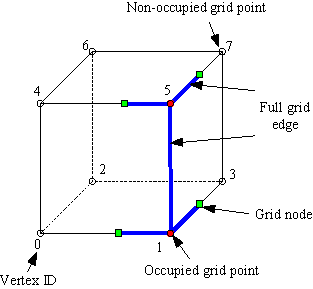
\includegraphics[width=0.5\textwidth]{images/tri_dexel_cell}
	\caption{
		A cell of a tri-dexel grid \cite{tridexel_reconstruction}.
		Occupied grid points are drawn in red, dexel nodes in green, dexel segments in blue.
		Each grid point is referenced using a number between 0 and 7 and has a list of neighboring grid points in counter-clockwise order, \cf left table.
	}
	\label{fig:tri_dexel_cell}
\end{figure}
%
Before a cell can be triangulated, a few consistency checks and corrections are applied to the cell.
This process is called regularization and ensures a successful triangulation into a water-tight mesh.
After ensuring the consistency of a cell, it can be triangulated.
For this purpose, a depth-first search process is iteratively started at non-occupied grid points of the cell to discover boundary loops.
Basically, the found loops can be triangulated right away to obtain a water tight mesh.
However, the quality of the triangulation can be further enhanced by taking normal information at the dexel nodes into account.
This is especially necessary to reconstruct features of the model.
This optional feature reconstruction pass is run on the loops found in the previous step and may create additional vertices.

\section{Implementation}
\label{sec:tri_dexel_implementation}

In order to run the tri-dexel surface reconstruction, the user must supply a resolution as parameter.
This resolution determines the size of the raycasted dexel images as well as the resulting tri-dexel grid.
For esthetic reasons, the specified resolution is only used for the longest dimension of the workpiece.
The resolution along the other dimensions is usually smaller in order to make the cells more cubic, although the implementation does not require cubic cells.


In addition to the types already specified by the VML, \cf figure \ref{fig:vml_datamodel}, the tri-dexel reconstruction algorithm requires a few more types.
Most of these type definitions and also the algorithms themselves are vastly simplified when compared with the underlying source code.
Especially parallelism, asynchrony, memory efficient handling of data structures and numeric stability enhancements have been intentionally left out in the discussed pseudo code.
The additional types needed for the tri-dexel implementation are shown in the class diagram in figure \ref{fig:tri_dexel_datamodel}.
%
\begin{figure}
	\centering
	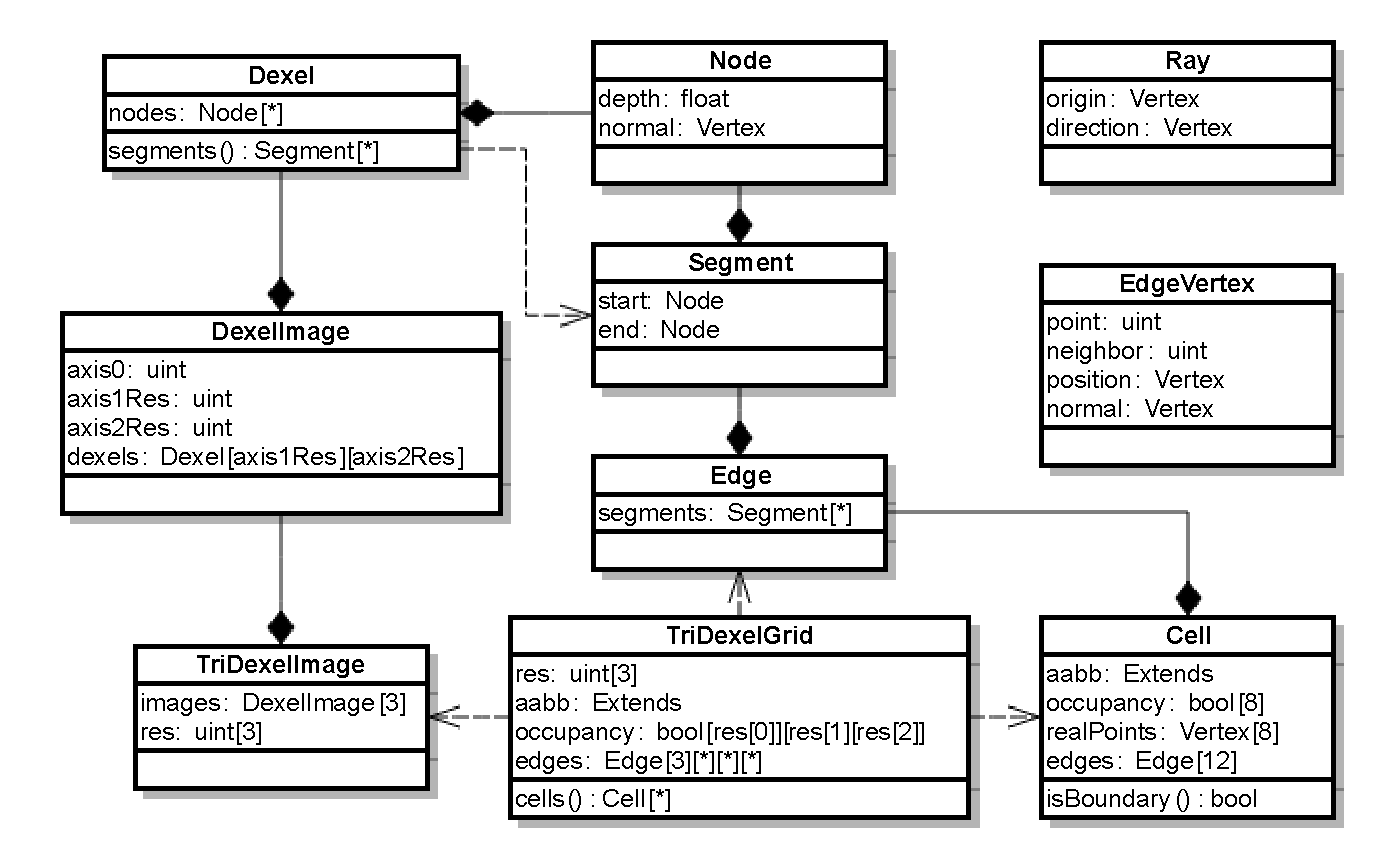
\includegraphics[width=0.9\textwidth]{images/tri_dexel_datamodel}
	\caption{
		Simplified UML class diagram of the types needed for the tri-dexel reconstruction algorithm in addition to the types used by the VML, \cf figure \ref{fig:vml_datamodel}.
	}
	\label{fig:tri_dexel_datamodel}
\end{figure}
%
The most central data structure is the \var{TriDexelGrid} class.
It represents a tri-dexel representation of the complete VML workpiece which is already prepared for subsequent regularization and triangulation.
In addition to the tri-dexel grid's resolution \var{res} and bounding box \var{aabb}, the \var{TriDexelGrid} class further contains the occupancy information for each grid point in \var{occupancy}, \ie whether a grid point is spanned by a dexel or not, as well as the actual dexel segments between the grid points, stored in \var{edges}.
The \var{cells} method separates all this information into distinct and independent cells.
Each cell is an instance of the \var{Cell} class and contains the same information as the tri-dexel grid, but locally for a single cell.
A cell stores it's bounding box \var{box}, the point occupancy of each of the cell's corners in \var{occupancy}, the corners' coordinates in \var{realPoints} and the 12 edges of the cell, stored in \var{edges}.
Each edge of the cell is an instance of \var{Edge} and contains all spanning dexel segments, clamped to the interval between the edge's incident grid points.
Furthermore, a method \var{isBoundary} is provided to check if the cell is a boundary cell, \ie contains occupied and non-occupied grid points and therefore contains a part of the workpiece's surface.
The \var{TriDexelGrid} is constructed from the \var{TriDexelImage} class, which, fundamentally, contains the same information as the tri-dexel grid.
The difference is substantially clearer from the workflow's point of view.
Whereas the \var{TriDexelGrid} is already prepared for further processing, the \var{TriDexelImage} class only contains the raw result as created by raycasting the VML's data model from three orthogonal directions.
This data only consists of the resolution \var{res} used for raycasting as well as three dexel images \var{images} along the three coordinate system axes.
A \var{DexelImage} describes the result of a single raycast along the axis specified in \var{axis0}, where 0 denotes the x-, 1 the y- and 2 the z-axis.
The members \var{axis1Res} and \var{axis2Res} store the resolution of the dexel image along the two cyclically following axes after \var{axis0}.
For example, if \var{axis0} is 1, the y-axis, then \var{axis1Res} and \var{axis2Res} hold the resolutions along the axes 2 and 0, the z- and x-axis.
Finally, \var{dexels} contains all the dexels of the image.
Each \var{Dexel} instance is then essentially a list of nodes, stored in \var{nodes}.
The number of stored nodes after raycasting is always a multiple of two.
As dexel nodes are typically processed in pairs, as dexel segments, a convenience method \var{segments} is provided which groups adjacent nodes into instances of \var{DexelSegment}.
A \var{DexelSegment} contains these two nodes as \var{start} and \var{end} node.
Finally, the \var{Node} class holds the depth of the node along its dexel, \ie the distance of the node from the plane where the dexels originate, \cf figure \ref{fig:dexel_image}, as well as the normal vector of this surface entry/exit.
Unrelated to the tri-dexel types is the additional class \var{Ray} which represents a ray starting at the vertex \var{origin} and traveling into the direction stored by \var{direction}.

Based on the discussed tri-dexel types, the basic reconstruction algorithm is shown in algorithm \ref{alg:tri_dexel}.
%
\begin{algorithm}
	\centering
	\begin{algorithmic}[1]
		\Function{TriDexel}{$\var{grid}, \var{resolution}$}
			\State $\var{box} = \var{Extends}(\var{grid}.\var{aabb}.\var{lower} - \epsilon, \var{grid}.\var{aabb}.\var{upper} + \epsilon)$
			\State $\var{res} = \Call{UniformResolution}{\var{box}, \var{resolution}}$
			\State $\var{img} = \var{TriDexelImage}(\var{res})$
			\State $\Call{AxisParallelRaycast}{\var{grid}, \var{box}, \var{res},\hfill\break
				\hspace*{\dimexpr\algorithmicindent*2}(\var{axis}, \var{x}, \var{y}, \var{v}, \var{n}) \rightarrow \var{img}.\var{images}_{\var{axis}}.\var{dexels}_{\var{x}, \var{y}}.\var{nodes}.\var{add}(\var{Node}(\var{v}_{\var{axis}}, \var{n}))}$
			\State $\var{dgrid} = \Call{CreateTriDexelGrid}{\var{img}, \var{box}}$
			\State $\var{triangles} \gets \varnothing$
			\ForAll{$\var{c} \in \var{dgrid}.\var{cells}()$}
				\State $\Call{RegularizeCell}{\var{c}}$
				\State $\var{triangles} \gets \var{triangles} \cup \Call{TriangulateCell}{\var{c}}$
			\EndFor
			\State \Return $\var{triangles}$
		\EndFunction
	\end{algorithmic}
	\caption{
		Abstract workflow of the surface reconstruction using a tri-dexel approach.
	}
	\label{alg:tri_dexel}
\end{algorithm}
%
At the beginning, a slightly enlarged bounding box is calculated for the size of the tri-dexel grid and raycast.
In this way, edge cases with a surface exactly at the grid's border are avoided.
The \textproc{UniformResolution} function takes the user-specified resolution and the tri-dexel grid's bounding box and calculates three resolutions, one for each axis.
The longest one is equal to the specified resolution and the other two are calculated in such a way that the resulting cells of the tri-dexel grid are as cubic as possible.
This resolution is used to preallocate space for the tri-dexel image which is then filled in the subsequent raycasting process.
The remaining part of the algorithm closely follows the concept discussed in the previous section\ref{sec:tri_dexel_concept}.
The subsequent sections discuss the functions and procedures of the algorithm in the order they are used.


\subsection{Raycast}
\label{sec:tri_dexel_raycast}

The raycast is the prime algorithm for converting the VML's data model into a tri-dexel representation.
The raycast is performed with parallel, axis-aligned and equidistant rays.
All rays start at the intersection points of a uniform 2-dimensional grid placed on one side of the data model's slightly enlarged bounding box and end at the opposite side, \cf figure \ref{fig:dexel_image}.
Three of these raycasts along the three axes of the coordinate system result in three dexel images.
As the raycasting code is kept separated from the tri-dexel data structures, a function is passed to the raycasting code which is invoked each time a ray has found a surface intersection.
Therefore, the same code can be used to create other data structures as well. %TODO: ref point cloud creation

The entry routine and ray creation code of the raycasting algorithm is shown in algorithm \ref{alg:tri_dexel_raycast}.
%
\begin{algorithm}
	\centering
	\begin{algorithmic}[1]
		\Procedure{Raycast}{$\var{grid}, \var{box}, \var{res}, \var{hitFunc}$}
			\For{$\var{axis0} \gets 0 \To 2$}
				\State $\var{axis1} \gets (\var{axis0} + 1) \bmod 3$
				\State $\var{axis2} \gets (\var{axis0} + 2) \bmod 3$
				\State $\var{xCount} \gets \var{res}_{\var{axis1}}$
				\State $\var{yCount} \gets \var{res}_{\var{axis2}}$
				\State $\Delta \var{x} \gets (\var{box}.\var{upper}_{\var{axis1}} - \var{box}.\var{lower}_{\var{axis1}}) \div (\var{xCount} - 1)$
				\State $\Delta \var{y} \gets (\var{box}.\var{upper}_{\var{axis2}} - \var{box}.\var{lower}_{\var{axis2}}) \div (\var{yCount} - 1)$
				\For{$\var{y} \gets 0 \To \var{yCount} - 1$}
					\For{$\var{x} \gets 0 \To \var{xCount} - 1$}
						\State $ray = \Call{CreateRay}{\var{box}, \var{axis0}, \var{axis1}, \var{axis2}, \var{\Delta x}, \var{\Delta y}, \var{x}, \var{y}}$
						\State $\Call{CastRay}{\var{grid}, \var{axis0}, \var{axis1}, \var{axis2}, \var{ray},\hfill\break
							\hspace*{\dimexpr\algorithmicindent*5}(\var{v}, \var{n}) \rightarrow \var{hitFunc}(\var{axis0}, \var{x}, \var{y}, \var{v}, \var{n})}$
					\EndFor
				\EndFor
			\EndFor
		\EndProcedure
		\\
		\Function{CreateRay}{$\var{box}, \var{axis0}, \var{axis1}, \var{axis2}, \var{\Delta x}, \var{\Delta y}, \var{x}, \var{y}, \var{xCount}, \var{yCount}$}
			\State $\var{origin} \gets \var{box}.\var{lower}$
			\State $\var{origin}_{axis1} \gets \var{origin}_{\var{axis1}} + \var{x} * \var{\Delta x}$
			\State $\var{origin}_{axis2} \gets \var{origin}_{\var{axis2}} + \var{y} * \var{\Delta y}$
			\State $\var{direction} = \var{Vertex}(0, 0, 0)$
			\State $\var{direction}_{\var{axis0}} \gets 1$
			\State \Return $\var{Ray}(\var{origin}, \var{direction})$
		\EndFunction
		\\
		\Procedure{CastRay}{$\var{grid}, \var{axis0}, \var{axis1}, \var{axis2}, \var{ray}, \var{hitFunc}$}
			\State $\var{traverser} \gets \var{AxisAlignedTraverser}(\var{grid}, \var{ray}, \var{axis0}, \var{axis1}, \var{axis2})$
			\While{$\neg \var{traverser}.\var{reachedEnd}()$}
				\State $\var{cell} \gets \var{traverser}.\var{nextCell}()$
				\State $\Call{IntersectCell}{\var{cell}, \var{ray}, \var{axis0}, \var{axis1}, \var{axis2}, \var{hitFunc}}$
			\EndWhile
		\EndProcedure
	\end{algorithmic}
	\caption{
		Basic algorithm for performing a parallel raycast along all three coordinate system axes on the VML's data model.
	}
	\label{alg:tri_dexel_raycast}
\end{algorithm}
%
The outmost procedure \textproc{Raycast} takes four arguments: the VML's regular grid data structure, the slightly enlarged bounding box of the raycasted area, the resolution of the raycasted \enquote{image} as well as a function, which is called on every surface hit.
The algorithm starts of by iterating over the three coordinate system's axes.
The index of each axis is stored in the variable \var{axis0}, where 0 denotes the x-, 1 the y- and 2 the z-axis.
\var{axis0} is also called primary axis and is accompanied by \var{axis1} and \var{axis2} which hold the other two, secondary axes, in cyclic order.
Depending on the choice of primary and secondary axes, the resolution of the 2-dimensional grid spawning the rays is determined and assigned to \var{xCount} and \var{yCount}, for the horizontal and vertical resolution.
Afterwards, the distance between two incident rays along both secondary axes is computed.
Therefore, along both secondary axes, the size of the bounding box is computed and divided by the resolution minus one.
The result is assigned to the variables \var{\Delta x} and \var{\Delta y}.
Now the algorithm starts creating and casting all rays along their primary axis.
Two nested loops iterate over all points of the 2-dimensional grid spawning rays.
For each grid point at $\var{x}, \var{y}$ a ray is created using the \textproc{CreateRay} function.
Subsequently, the ray is cast into the VML's regular grid by invoking \textproc{CastRay}, passing a closure which is invoked each time a hit is recorded.

The \textproc{CreateRay} function's objective is to create an instance of \var{Ray} storing the ray's origin and direction.
The origin is calculated by starting from the bounding box's \var{lower} corner.
Along the primary axis, this value is already correct.
On the secondary axes, the origin, currently at the origin for ray $0, 0$, must be moved according to the ray's \var{x} and \var{y} coordinate.
In order to do so, \var{x} and \var{y} are multiplied by the distances between incident rays, \var{\Delta x} and \var{\Delta y}, and added to the origin's secondary axes.
%
Computing the ray's direction is simpler, as it is axis aligned.
Therefore, the direction is a unit vector along the primary axis, created by setting the corresponding component of a zeroed vector to one.
%
Finally, \var{origin} and \var{direction} are aggregated into an instance of \var{Ray} and returned.

After rays have been created, they are cast into the VML's regular grid data structure to find surface intersections using the \textproc{CastRay} procedure.
Traversing a ray through a regular grid is usually done using the 3D-DDA algorithm \cite{3DDDA}, \cf figure \ref{fig:traverser}.
However, as the rays are axis parallel, traversal essentially boils down to mapping the ray's origin to the appropriate grid cell and incrementing the 3-dimensional cell index along the primary axis until the other end of the grid is reached.
This logic is hidden behind the \var{AxisAlignedTraverser} class and is no further elaborated.
%
The ray is then intersected with each cell pulled from the traverser using the \textproc{IntersectCell} algorithm.
Fundamentally, the implementation is based on the inside counting scheme of the visualization code explained in figure \ref{fig:raycast}.
The important difference is that the raycast for visualization may terminate after the first intersection found.
Furthermore, minor inconsistencies are tolerable and may result in a few pixel errors on the final image.
However, when creating dexels, a consistent number of surface entries and exits as well as numerically correct ordering of the intersections is substantial.
Consequently, such an intersection routine must employ a great deal of numeric precautions and extra checks to deliver a correct result, even sacrificing intersections for the sake of consistency.
This procedure forms the heart of the raycasting algorithm.
As it is quite comprehensive and highly tailored to the VML's internal data structures, the detailed pseudocode of the \textproc{IntersectCell} routine is omitted from the thesis.


\subsection{Tri-dexel image and grid generation}
\label{sec:tri_dexel_dexel_image_generation}

Based on the generic, axis parallel raycasting routine, a tri-dexel image is created in the base algorithm \ref{alg:tri_dexel}.
Before the raycast is lauched, an instance of \var{TriDexelImage} is created, preallocating enough space to hold 3 dexel images, each holding a 2-dimensional grid of empty dexels.
When calling \textproc{AxisParallelRaycast} procedure, an anonymous function is passed which is invoked on every surface hit detected during raycasting.
This function receives the primary axis \var{axis}, \ie the axis along the rays where traversed, \var{x} and \var{y} coordinate on the 2-dimensional dexel grid as well as the intersection point \var{v} with the normal of the hit triangle \var{n}.
With this information, the tri-dexel image stored in \var{img} is populated.
Once raycasting has completed, the tri-dexel grid is generated from the tri-dexel image.
This conversion is more a reinterpretation and preparation of the information contained within the tri-dexel image.
Whereas the image contains the raw raycasting result, the tri-dexel grid already stores grid point occupancy information and cuts all dexels at cell borders.
This preparation eases the follow-up processing of individual cells.

Converting the tri-dexel image into a tri-dexel grid is done by the \textproc{CreateTriDexelGrid} function, which is shown in algorithm \ref{alg:tri_dexel_grid_generation}.
%
\begin{algorithm}
	\centering
	\begin{algorithmic}[1]
		\Function{CreateTriDexelGrid}{$\var{triImg}, \var{box}$}
			\State $\var{res} = \var{triImg}.\var{res}()$
			\State $\var{grid} = \var{TriDexelGrid}(\var{res}, \var{box})$
			\For{$\var{axis0} \gets 0 \To 2$}
				\State $\var{axis1} \gets (\var{axis0} + 1) \bmod 3$
				\State $\var{axis2} \gets (\var{axis0} + 2) \bmod 3$
				\For{$\var{axis1Val} \gets 0 \To \var{res}_{\var{axis1}} - 1$}
					\For{$\var{axis2Val} \gets 0 \To \var{res}_{\var{axis2}} - 1$}
						\State $\var{dexel} \gets \var{triImg.images}_{\var{axis0}}.\var{dexels}_{\var{axis1Val}, \var{axis2Val}}$
						\ForAll{$\var{seg} \in \var{dexel}.\var{segments}()$}
							\LineComment{Compute affected grid point range}
							\State $\var{start} \gets \floor{\Call{MapDepthToGrid}{\var{seg}.\var{start}.\var{depth}, \var{axis0}, \var{res}, \var{box}}}$
							\State $\var{end} \gets \floor{\Call{MapDepthToGrid}{\var{seg}.\var{end}.\var{depth}, \var{axis0}, \var{res}, \var{box}}}$
							\For{$\var{axis0Val} \gets \var{start} \To \var{end}$}
								\State $\var{gridFrom}$
								\State $\var{gridFrom}_{\var{axis0}} \gets \var{axis0Val}$
								\State $\var{gridFrom}_{\var{axis1}} \gets \var{axis1Val}$
								\State $\var{gridFrom}_{\var{axis2}} \gets \var{axis2Val}$
								\State $\var{gridTo} \gets \var{gridFrom}$
								\State $\var{gridTo}_{axis0} \gets \var{gridTo}_{\var{axis0}} + 1$
								\State $\var{depthFrom} = \Call{MapGridToDepth}{\var{gridFrom}_{\var{axis0}}, \var{axis0}, \var{res}, \var{box}}$
								\State $\var{depthTo}   = \Call{MapGridToDepth}{\var{gridTo}_{\var{axis0}}, \var{axis0}, \var{res}, \var{box}}$
								\LineComment{Point occupancy}
								\If{$\var{seg}.\var{start}.\var{depth} \leq \var{depthFrom} \leq \var{seg}.\var{end}.\var{depth}$}
									\State $\var{grid}.\var{occupancy}_{\var{gridFrom}} \gets \True$
								\EndIf
								\If{$\var{seg}.\var{start}.\var{depth} \leq \var{depthTo} \leq \var{seg}.\var{end}.\var{depth}$}
									\State $\var{grid}.\var{occupancy}_{\var{gridTo}} \gets \True$
								\EndIf
								\LineComment{Copy and clamp to cell border}
								\State $\var{s} \gets \var{seg}$
								\If{$\var{s}.\var{start}.\var{depth} \leq \var{depthFrom}$}
									\State $\var{s}.\var{start}.\var{depth} \gets \var{depthFrom}$
								\EndIf
								\If{$\var{s}.\var{end}.\var{depth} \geq \var{depthTo}$}
									\State $\var{s}.\var{end}.\var{depth} \gets \var{depthTo}$
								\EndIf
								\State $\var{grid}.\var{edges}_{\var{axis0}, \var{gridFrom}}.\var{segments}.\var{add}(\var{s})$
							\EndFor
						\EndFor
					\EndFor
				\EndFor
			\EndFor
		\EndFunction
		\Function{MapDepthToGrid}{\var{depth}, \var{axis0}, \var{res}, \var{box}}
			\State \Return $(\var{depth} - \var{box}.\var{lower}_{\var{axis0}}) \div (\var{box}.\var{upper}_{\var{axis0}} - \var{box}.\var{lower}_{\var{axis0}}) * (\var{res}_{\var{axis0}} - 1)$
		\EndFunction
		\Function{MapGridToDepth}{\var{gridCoord}, \var{axis0}, \var{res}, \var{box}}
			\State \Return $\var{gridCoord} \div (\var{res}_{\var{axis0}} - 1) * (\var{box}.\var{upper}_{\var{axis0}} - \var{box}.\var{lower}_{\var{axis0}}) + \var{box}.\var{lower}_{\var{axis0}}$
		\EndFunction
	\end{algorithmic}
	\caption{
		Creating a tri-dexel grid from the raycasted dexel images.
	}
	\label{alg:tri_dexel_grid_generation}
\end{algorithm}
%



\subsection{Regularization}
\label{sec:tri_dexel_regularization}

\begin{figure}
	\centering
	\includegraphics[width=0.9\textwidth]{images/tri_dexel_regularization}
	\caption{
		The four regularization rules applied to each tri-dexel cell before it is triangulated \cite{tridexel_reconstruction}.
	}
	\label{fig:tri_dexel_regularization}
\end{figure}


\begin{algorithm}
	\centering
	\begin{algorithmic}[1]
		\Function{RegularizeCell}{$\var{c}$}
		
		\EndFunction
	\end{algorithmic}
	\caption{
		Regularizing a cell of the tri-dexel grid by applying the four rules specified in figure \ref{fig:tri_dexel_regularization} \cite{tridexel_reconstruction}.
	}
	\label{alg:tri_dexel_regularization}
\end{algorithm}


\subsection{Triangulation}
\label{sec:tri_dexel_triangulation}

For this purpose, a depth-first search process is iteratively started at non-occupied grid points of the cell.
The search traverses the cell's edges and backtracks each time an occupied grid point and therefore a grid edge containing a dexel node is found.
The list of visited grid edges containing dexel nodes, in the order they where visited, forms a boundary loop.
A cell might contain multiple boundary loops, found when starting at different, non-occupied grid points.

\begin{figure}
	\centering
	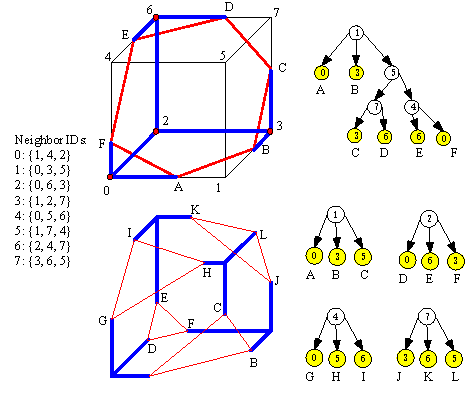
\includegraphics[width=0.9\textwidth]{images/tri_dexel_triangulation}
	\caption{
		Triangulating a tri-dexel cell by finding boundary loops using depth-first search along the cube, starting at non-occupied nodes \cite{tridexel_reconstruction}.
	}
	\label{fig:tri_dexel_triangulation}
\end{figure}

\begin{algorithm}
	\centering
	\begin{algorithmic}[1]
		\Function{TriangulateCell}{$\var{c}$}
		
		\EndFunction
	\end{algorithmic}
	\caption{
		Basic triangulating routine for a tri-dexel cell.
		No refinement or feature reconstruction is done.
	}
	\label{alg:tri_dexel_triangulation}
\end{algorithm}

\subsection{Refinement and feature reconstruction}
\label{sec:tri_dexel_refinement}

This optional feature reconstruction pass is run on the loops found in the previous step.
Using the normals of each pair of adjacent dexel nodes of the loop, an additional intermediate/feature point may be created.
Using the normals of multiple nodes, a further apex vertex may be created per loop.
Finally, these enhanced loops are also triangulated.

\begin{figure}
	\centering
	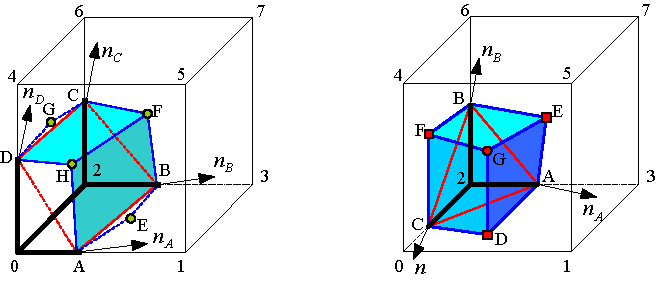
\includegraphics[width=0.9\textwidth]{images/tri_dexel_refinement}
	\caption{
		Triangulating a tri-dexel cell by finding boundary loops using depth-first search along the cube, starting at non-occupied nodes \cite{tri_dexel_refinement}.
	}
	\label{fig:tri_dexel_refinement}
\end{figure}


\subsection{Subslicing *experimential*}
\label{sec:tri_dexel_subslicing}



\subsection{Parallelization}
\label{sec:tri_dexel_parallelization}

raycast, parallel cell processing


\section{Results}
\label{sec:tri_dexel_results}


